%%%%%%%%%%%%%%%%%%%%%%%%%%%%%%%%%%%%%%%%%%%%%%%%%%%%%%%%%%%%%%%%%%%%%%%%%%%%%%%%%%%%%%%%%%%%%%%%%
%
% Document:     DM Support Prd.  product tree
%
%%%%%%%%%%%%%%%%%%%%%%%%%%%%%%%%%%%%%%%%%%%%%%%%%%%%%%%%%%%%%%%%%%%%%%%%%%%%%%
\documentclass{article}
\usepackage{times,layouts}
\usepackage{tikz,hyperref,amsmath}
\usetikzlibrary{positioning,arrows,shapes,decorations.shapes,shapes.arrows}
\usetikzlibrary{backgrounds,calc}
\usepackage[paperwidth=444pt,paperheight=172pt,
left=-2mm,top=3mm,bottom=0mm,right=0mm,
noheadfoot,marginparwidth=0pt,includemp=false,
textwidth=30cm,textheight=50mm]{geometry}
\newcommand\showpage{%
\setlayoutscale{0.5}\setlabelfont{\tiny}\printheadingsfalse\printparametersfalse
\currentpage\pagedesign}
\hypersetup{pdftitle={DM products }, pdfsubject={Diagram illustrating the
                products in LSST DM }, pdfauthor={Autogenerated from MD}}
\tikzstyle{tbox}=[rectangle,text centered, text width=30mm]
\tikzstyle{wbbox}=[rectangle, rounded corners=3pt, draw=black, top color=blue!50!white,
                    bottom color=white, very thick, minimum height=40pt, inner sep=2pt,
                    text centered, text width=30mm]
\tikzstyle{pbox}=[rectangle, rounded corners=3pt, draw=black, top
 color=yellow!50!white, bottom color=white, very thick,
 minimum height=36pt, inner sep=3pt, text centered, text width=35mm]
\tikzstyle{pline}=[-, thick]
\begin{document}
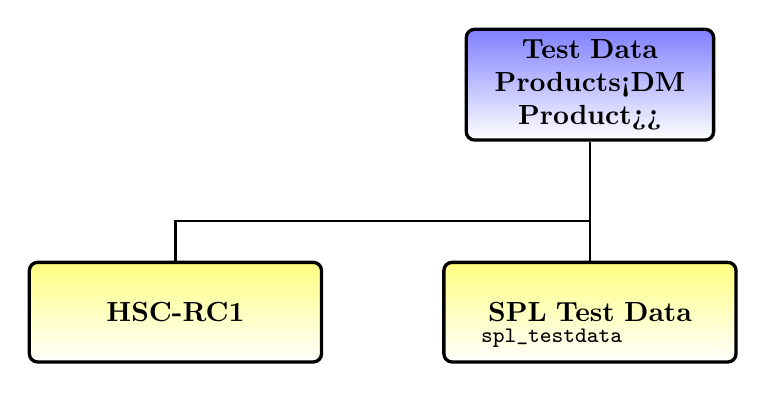
\begin{tikzpicture}[node distance=0mm]


\node (HSCRC1) [pbox, 
] {\textbf{HSC-RC1
} };\node [below right] at (HSCRC1.north west) {\footnotesize \color{blue}} ;

\node (SPLTD) [pbox, 
right=43pt of HSCRC1] {\textbf{SPL Test Data
} };\node [below right] at (SPLTD.north west) {\footnotesize \color{blue}} ;
\node (SPLTDpkg) [tbox,below=3mm of SPLTD.north] {{\footnotesize \color{black} \begin{verbatim} spl_testdata \end{verbatim} }  };

\node (DMDTDP) [wbbox, above=43pt of SPLTD]{\textbf{Test Data Products<DM Product>>}};
 \draw[pline]   (HSCRC1.north) -- ++(0.0,0.5) -| (DMDTDP.south) ; 
 \draw[pline]   (SPLTD.north) -- ++(0.0,0.5) -| (DMDTDP.south) ; 

\end{tikzpicture}
\end{document}
